\documentclass[a4paper,12pt]{report}
\usepackage[slovak,english]{babel}
\usepackage[utf8]{inputenc}   
\usepackage[protrusion=true,expansion=true]{microtype} 
\usepackage{mathpazo}
\usepackage[T1]{fontenc}             
\linespread{1.5}
%alebo cez \renewcommand{\baselinestretch}{1.5}\normalsize
\usepackage{moresize}
\usepackage{geometry} 
%\usepackage[inner=4cm,outer=2cm,bottom=2.5cm]{geometry} 
\addtolength{\oddsidemargin}{-.5cm}
\addtolength{\evensidemargin}{-2.9cm}   
\addtolength{\topmargin}{0cm}
\addtolength{\textheight}{0cm}
\addtolength{\textwidth}{2.cm}
\addtolength{\textheight}{2.cm}
\usepackage{graphicx}
\usepackage{hyperref, fancyhdr}
\usepackage{float}
\usepackage{subfig}
\usepackage{pdfpages}
\usepackage{listings}
\usepackage{eurosym}
\usepackage{url,mathptmx} 
\usepackage{booktabs}
\usepackage{array, hhline} 
\usepackage{lscape}
\usepackage{amssymb, amsmath, amsfonts, lmodern}
%\usepackage{amssymb, amsmath, lmodern}
%toto je trochu ine pismo \usepackage{amssymb,amsfonts,amscd}
\usepackage{acronym}
\usepackage{paralist}
\usepackage{verbatim}	
\usepackage{comment}
\usepackage[colorinlistoftodos]{todonotes}
\usepackage[pdftex,unicode,bookmarks=false]{hyperref}
\usepackage{fancyhdr}
\usepackage{csquotes}
\usepackage{makecell}

\renewcommand{\chaptermark}[1] %	HEADER / FOOTER  DEFINITIONS
{
  \markboth{#1}{}
}
\usepackage{sectsty}%	SECTION TITLE APPEARANCE
\allsectionsfont{\mdseries\upshape} 
\usepackage[explicit]{titlesec}
\usepackage[nottoc,notlof,notlot]{tocbibind} 
\usepackage[titles,subfigure]{tocloft}
\renewcommand{\cftsecfont}{\rmfamily\mdseries\upshape}
\renewcommand{\cftsecpagefont} {\rmfamily\mdseries\upshape}

\usepackage{nicefrac}
\usepackage{biblatex}

\addbibresource{literatura.bib} 

\newtheorem{mydef}{Definícia}
\newtheorem{myexample}{Príklad}


\fancypagestyle{plain}{%
  \fancyhf{}%
  \fancyhead[L, R]{SPŠD TT \hfill STREDOŠKOLSKÁ ODBORNÁ ČINNOSŤ }
   \fancyfoot[C]{}
   \fancyfoot[R]{\thepage}
}
 \renewcommand{\headrulewidth}{0pt} % remove lines as well

\titlespacing*{\chapter}{0pt}{-30pt}{30pt}

\titleformat{\section}{\LARGE\bf}{\textcolor{black}{\thesection\hspace{12pt} #1}}{0pt}{}
\titleformat{\subsection}{\large\bf}{\textcolor{black}{#1}}{0pt}{}


\begin{document}
  \selectlanguage{slovak}
  \titleformat{\chapter}[display]{\normalfont\bfseries}{}{10pt}{\huge#1}





  \pagestyle{empty}

  \begin{titlepage}
    \phantom.
    
    \begin{center}
    {\sc\LARGE Stredná priemyselná škola dopravná v Trnave}
    \medskip
   
    {\sc\large Študentská 23, 917 45 Trnava}
    \break
    \end {center}
    \vspace{6.5cm}
    
    
    \begin{center}
    {\sc\LARGE Návrh a implementácia smart-meteo stanice}
    \break
    {\sc\LARGE\bf Stredoškolská odborná činnosť}
    
    \medskip
    \end{center}
    
    
    
    \vspace{5cm}
    
    
    
    \phantom.\hfill
    
    \vfill
    \sc\large \textbf{2023} \hfill\sc\large\textbf{Filip Majchrák}
    
    \phantom.
    \end{titlepage}
  \begin{titlepage}
    \phantom.
    
    \bigskip
    
    \begin{center}
    {\sc\LARGE Stredná priemyselná škola dopravná Trnava}
    \bigskip
    
    {\sc\large Študentská 23, 917 45 Trnava}
    \break
    \end{center}
    \vspace{4.5cm}
    
    \begin{center}
    
    {\sc\Large{\bf Návrh a implementácia smart meteo stanice\\}}
    \medskip
    {\sc\large Stredoškolská odborná činnosť}
    
    \end{center}
    
    
    \vspace{3cm}
    
    
    
    \phantom.\hfill
    
    {\noindent\sc\small\bf číslo odboru: 2675M\\}
    {\sc\small\bf Názov odboru: Elektrotechnika - komunikačné a sieťové technológie \\}
    {\sc\small\bf Školiteľ: Ing. Vladimír Brath\\ }
    {\sc\small\bf Ročník štúdia: štvrtý\\ }
    
    \medskip
        
    \large\bf Trnava 2023
    \hfill
    \large\bf Filip Majchrák
    
    \hfill\phantom.
    
    %\vspace{1.7cm}
    
    \phantom.
    \end{titlepage}
  %naskenovat a pridat do priecinka
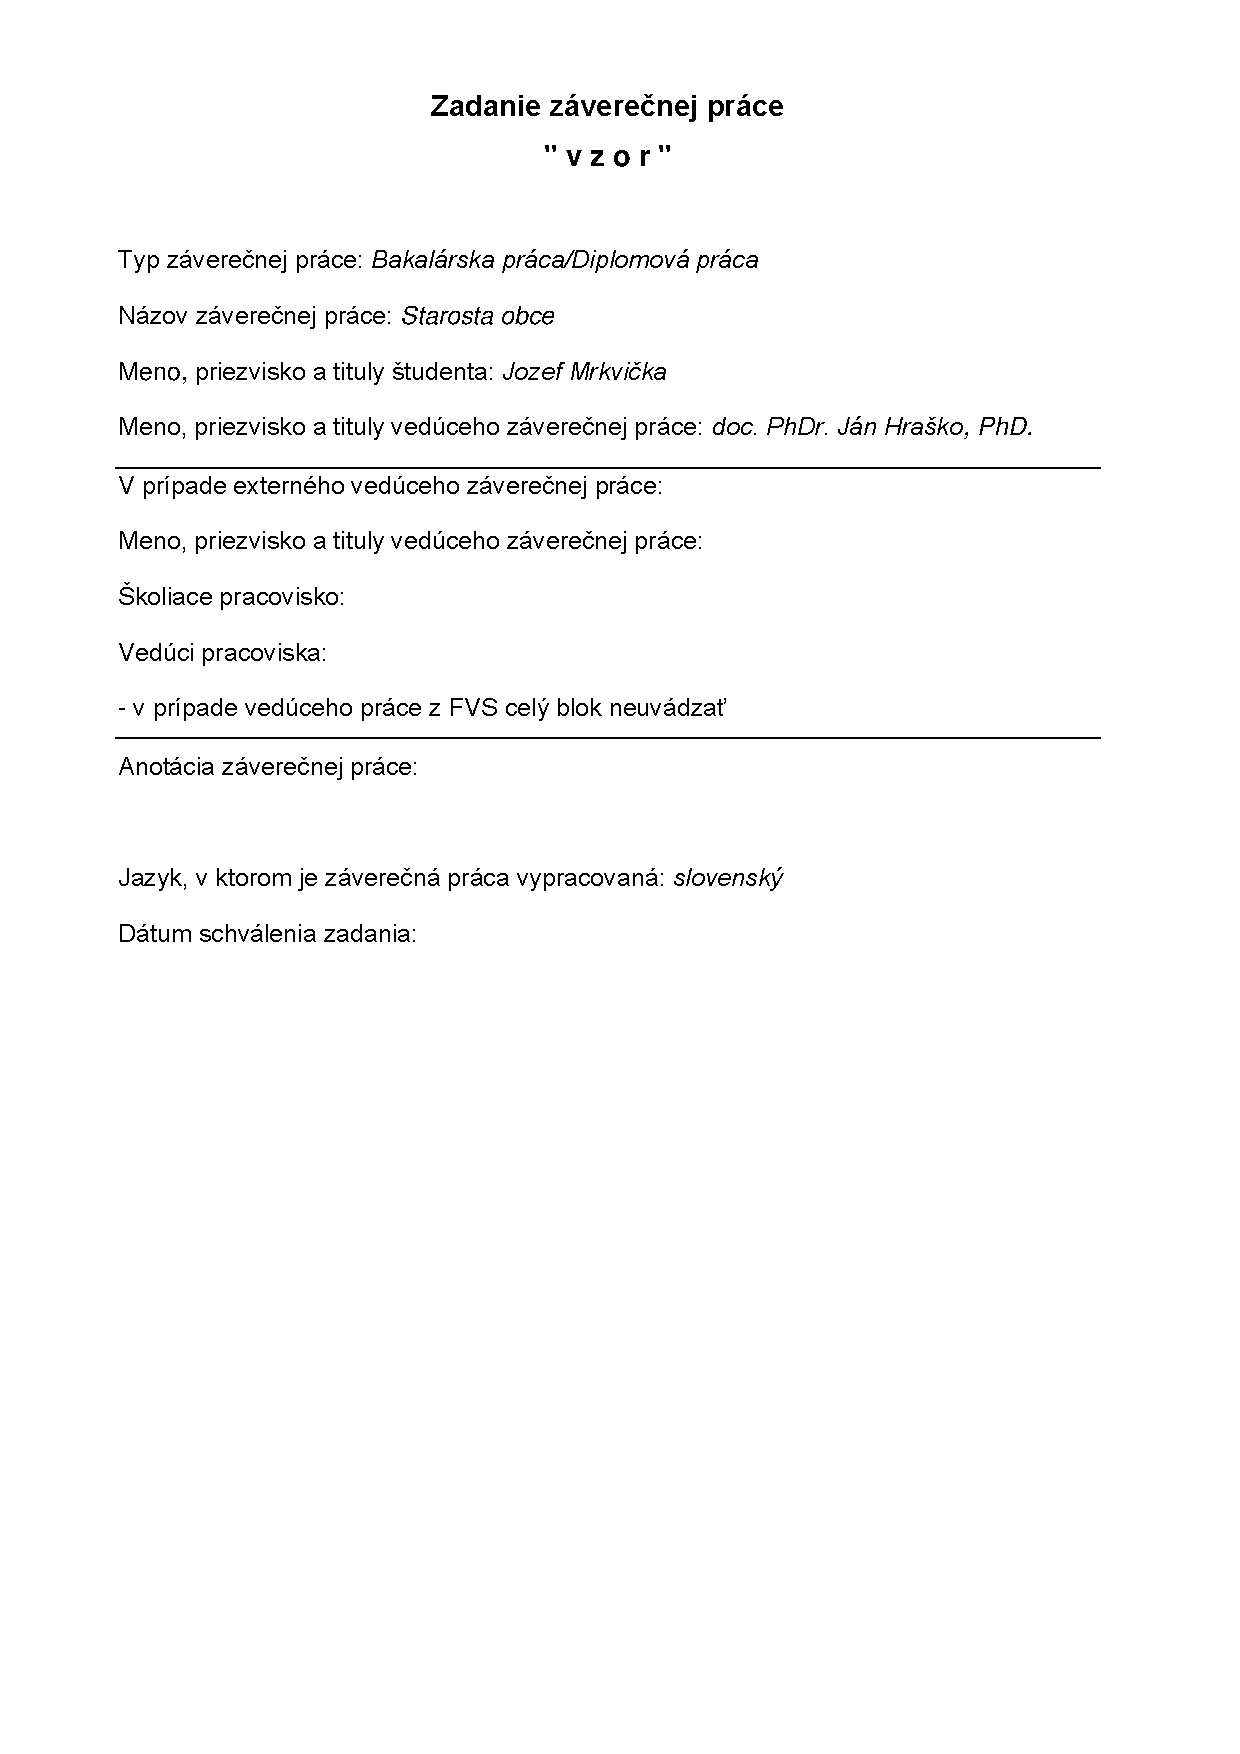
\includepdf{obrazky/Šablóna zadania záverečnej práce.pdf}   %toto odkomentovat pri tlaceni, alebo ked tam budete mat naskenovane zadanie, alebo 


  \pagestyle{plain}
  \setcounter{page}{3}

  \setcounter{secnumdepth}{5}
  \newpage
\phantom.
\vspace{12cm}
\noindent{\bf Čestné vyhlásenie}

\vspace{2em}

Čestne prehlasujem, že bakalársku prácu na tému \textit{Návrh a implementácia informačného systému doRest} som vypracoval samostatne s použitím všetkých dostupných poznatkov z doterajšieho štúdia, a uvedenej literatúry, ktorá je uvedená v zozname bibliografických odkazov. Predkladanú prácu som vykonával pod odborným vedením konzultanta doc. Ing. Michala Kebíska PhD.


\vspace{2em}

\noindent
V~Trnave, dňa ..............
\hfill
..........................................


\hfill
Bc. Samuel Domin \qquad\quad

  \newpage
\phantom.
\vspace{12cm}
\noindent{\bf Poďakovanie}
\vspace{2em}
\bigskip
\noindent

Na tomto mieste by som chcel poďakovať vedúcemu diplomovej práce doc. Ing. Michalovi Kebískovi PhD.  za cenné pripomienky a odborné rady, ktorými prispel k vypracovaniu tejto diplomovej práce. Taktiež ďakujem mojim kolegom za cenné rady pri analyzovani projektu. Zároveň ďakujem mojej rodine a priateľom za ich nekonečnú podporu a trpezlivosť. 

\vspace{2em}
  \fancyhead[L, R]{SPŠD TT \hfill STREDOŠKOLSKÁ ODBORNÁ ČINNOSŤ }

%--------------------------------------------------------------------------------------
%%% slovensky abstrakt
\noindent{\textbf{ABSTRAKT V ŠTÁTNOM JAZYKU }}
\\

\noindent
PRIEZVISKO, Meno: Názov témy záverečnej práce. [Bakalárska práca]. – Žilinská Univerzita v~Žiline. Fakulta riadenia a informatiky; Katedra informatiky. – Školiteľ/Vedúci: Ing. Oľga Chovancová –   Stupeň odbornej kvalifikácie: magister. – Mesto: FRI UNIZA, 20xx. Počet strán (napr. 35 s.)

\bigskip
Cieľom bakalárskej práce je ...

% \textit{Vzorové osnovy písania abstraktu:}
% Práca prezentuje... Objektom skúmania našej práce bolo... V práci analyzujeme... Vypracovali
% sme návrh... Overili sme postup... Predpokladá sa... Zistili sme... Navrhujeme aplikovať do
% praxe... .
% alebo:
% % 
% Cieľom záverečnej práce bolo... Práca je rozdelená do ... kapitol. Obsahuje ... grafov, ...
% tabuliek a ... príloh. Prvá kapitola je venovaná... V ďalšej časti sa charakterizuje... Záverečná
% kapitola sa zaoberá... Výsledkom riešenia danej problematiky je... .
% a pod.

\bigskip
\noindent
\textbf{Kľúčové slová}:  kľúčové slovo 1, kľúčové slovo 2, kľúčové slovo 3, ... kľúčové slovo x.
\bigskip
\\

\bigskip
\noindent\textbf{ABSTRAKT V CUDZOM JAZYKU }

\bigskip
The aim of the thesis is to .......

\bigskip
\noindent
\textbf{Key words: } key word 1, key word 2, key word 3,..., key word x. 

 %\lhead{FRI UNIZA}
 %\rhead{BAKALÁRSKA PRÁCA}
% \rfoot{\thepage}
\fancyhead[L, R]{SPŠD TT \hfill STREDOŠKOLSKÁ ODBORNÁ ČINNOSŤ }
% \fancyfoot[C]{}

\pagenumbering{arabic}
\addcontentsline{toc}{chapter}{Obsah}
\setcounter{tocdepth}{5}
\tableofcontents
\cleardoublepage
\newpage
\cleardoublepage
\listoffigures
\addcontentsline{toc}{chapter}{Zoznam obrázkov}
\listoftables
\addcontentsline{toc}{chapter}{Zoznam tabuliek}
\cleardoublepage
\pagestyle{plain}
\addcontentsline{toc}{chapter}{Zoznam skratiek}
\vspace{0pt plus 2cm}
\chapter*{Zoznam skratiek}
\begin{acronym}
    \acro{UML}{Unified Modelling Language}
\end{acronym}

%pouzitie v texte 
% \ac{SKRATKA} - long description (SKRATKA) 
% \ac{SKRATKA} - short - because it is second use 
% \acs{SKRATKA} - short  - this will force short form


%\pagenumbering{arabic}
\pagestyle{fancy}

%\include{kapitoly/uvod}	
\titleformat{\chapter}[display]{\normalfont\bfseries}{}{10pt}{\huge\thechapter\quad#1}

 %Pripadne doplniť dalsie kapitoly kde vytvoris novy subor
\chapter{Úvod}

 %sem vpis cokolvek chces. :) len tieto dve veticky mi prosim nechaj.

Celá dokumentácia je napísaná v typografickom systéme \LaTeX, ktorý ako formátovací jazyk používa počítačový program \TeX  vyvinutý Donaldom E. Knuthom.
\chapter{Teoreticky rozbor}
sddsdsds	
\chapter{Praktická realizácia}
V nasledujúcich podkapitolách si bližšie popíšeme proces realizácie. Ten je však rozdelený na viacero častí. V prvom rade bolo potrebné navrhnúť hardvér. V neskorších fázach softvér. Vo fáze vývoju softvéru sme používali agilnú metodiku bližšie metodiku V, ktorej presný popis je v obrázku.

\begin{figure}[h!]
    \centering
    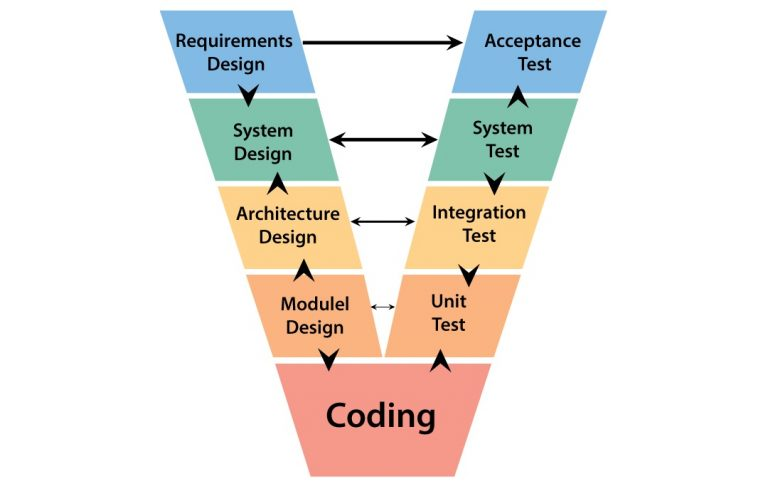
\includegraphics[width=0.6\textwidth]{obrazky/V_model.jpg}
    \caption{V metodika vývoju softvérového produktu}
\end{figure}
Na ľavej strane je vždy vývojový stupeň a na pravej strane je test, ktorý musí prebehnúť k danému vývojovému stupňu. Uprostred je fáza kódovania. 

\section{Hardvérová čast}
% TODO sem vpis podkapitoly kde blizsie popises o tvoreni dosiek
\section{Softvérová čast}
\subsection{Verzovanie súborov}
Všetky programy na ktorých sme pracovali boli uložené vo vzdiaľenom repozitári na serveri GitHub. GitHub je poskytovateľom internetového hostingu na vývoj softvéru a správu verzií s použitím verziovacieho nástroja Git. Ponúka distribuované verziovanie a správu zdrojového kódu systémom Git, ale aj ďalšie vlastné funkcie. Umožňuje regulovať prístup a má niekoľko funkcií zameraných na spoluprácu, ako napríklad sledovanie hlásených chýb, požiadavky na nové funkcie, správa úloh, priebežná integrácia a wiki stránka pre každý projekt.
%https://sk.wikipedia.org/wiki/GitHub
\subsection{Analýza}
Proces analýzy bol celý navrhnutý v programe Enterprise Architect. Kde sme používali \acs{UML} diagramy. Tam sme navrhli celú databázu a vyhľadali sme prípady použitia. Ku ktorým sme zapísali konkrétne scenáre ich aletrnatívy resp. sme použili aj diagramy aktivít. 
\subsection{FrontEnd}

\subsection{BackEnd}

\subsection{Databáza}
Na ukladanie zozbieraných hodnôt zo senzorov sme použili databázu. V našom prípade sa jednalo o databázu spoločnosti Oracle s názvom MySQL, ktorá je voľne dostupná a používa ju aj hosting kde je nasadený frontEnd.
\begin{figure}[h!]
    \centering
    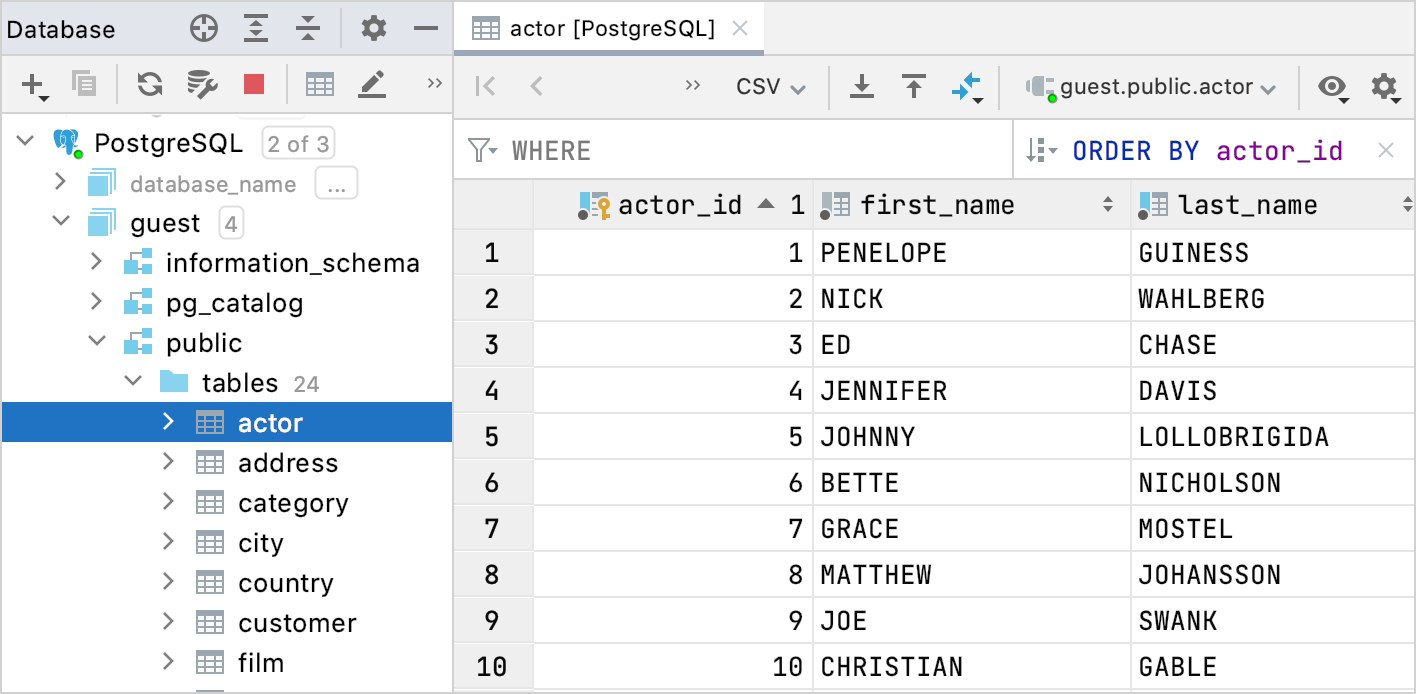
\includegraphics[width=0.6\textwidth]{obrazky/Table.png}
    \caption{Príklad databázovej tabuľky}
\end{figure}

\subsubsection{Návrhová čast databázy}
Pred samotným implementovaním frontEndu je dôležité si určiť podobu databázy. Databázy sa skladajú
\begin{itemize}
    \item tabuľky   
     \item stĺpce
     \item riadky
     \item primárne kľúče
     \item cudzie kľúče
\end{itemize} 
Preto si musíme prejsť celou návrhovou etapou databázy. Tá sa skladá z pomenovania problémových častí. Následne všetky vytypované problémy musíme roztriediť podľa vyššie spomínaného zoznamu.	
\chapter{Zaver}

sddsdsds

\titleformat{\chapter}[display]{\normalfont\bfseries}{}{10pt}{\huge#1}
%\include{kapitoly/zaver}

\renewcommand{\bibsection}{\chapter{Zoznam použitej literatúry}}
\addcontentsline{toc}{chapter}{Zoznam použitej literatúry}
\nocite{*}  %sluzi pre debugovanie, zakomentovat
\printbibliography[title=Zoznam použitej literatúry]

%\include{prilohy/zoznam_priloh}

 %Pripadne doplniť dalsie
\include{prilohy/priloha1}
%\include{prilohy/priloha2}
%\include{prilohy/priloha3}

\end{document}
